\documentclass[12pt,a4paper]{report}

% ==============================================================================
% CẤU HÌNH GÓI & NGÔN NGỮ TIẾNG VIỆT CHO OVERLEAF / PDFLATEX
% ==============================================================================
\usepackage[utf8]{inputenc}
\usepackage[vietnamese]{babel}
\usepackage[T5,T1]{fontenc}
\usepackage{lmodern}
\usepackage[a4paper,top=25mm,bottom=25mm,left=30mm,right=20mm]{geometry}
\usepackage{setspace}
\setstretch{1.25} % Giãn dòng 1.25 chuẩn tài liệu kỹ thuật

% ==============================================================================
% GÓI BỔ TRỢ HÌNH ẢNH, BẢNG BIỂU & TOÁN HỌC
% ==============================================================================
\usepackage{graphicx}
\usepackage{booktabs}
\usepackage{tabularx}
\usepackage{multirow}
\usepackage{array}
\usepackage{amsmath,amssymb}
\usepackage{caption}
\usepackage{subcaption}
\usepackage{float}
\usepackage{microtype}

% ==============================================================================
% MÀU SẮC & GÓI TÔ MÀU MÃ NGUỒN (LISTINGS)
% ==============================================================================
\usepackage{xcolor}
\definecolor{codegreen}{rgb}{0,0.6,0}
\definecolor{codegray}{rgb}{0.5,0.5,0.5}
\definecolor{codepurple}{rgb}{0.58,0,0.82}
\definecolor{backcolour}{rgb}{0.96,0.97,0.98}
\definecolor{darkblue}{rgb}{0.0,0.2,0.6}

\usepackage{listings}
\lstdefinestyle{mystyle}{
    backgroundcolor=\color{backcolour},   
    commentstyle=\color{codegreen}\itshape,
    keywordstyle=\color{magenta}\bfseries,
    numberstyle=\tiny\color{codegray},
    stringstyle=\color{codepurple},
    basicstyle=\ttfamily\footnotesize,
    breakatwhitespace=false,         
    breaklines=true,                 
    captionpos=b,                    
    keepspaces=true,                 
    numbers=left,                    
    numbersep=6pt,                  
    showspaces=false,                
    showstringspaces=false,
    showtabs=false,                  
    tabsize=2,
    frame=single,
    rulecolor=\color{black!20}
}
\lstset{style=mystyle}

% Định nghĩa ngôn ngữ bổ sung cho listings nếu cần
\lstdefinelanguage{yaml}{
  keywords={true,false,null,y,n},
  keywordstyle=\color{darkblue}\bfseries,
  basicstyle=\ttfamily\footnotesize,
  sensitive=false,
  comment=[l]{\#},
  morecomment=[s]{/*}{*/},
  commentstyle=\color{codegreen}\ttfamily,
  stringstyle=\color{codepurple}\ttfamily,
  moredelim=[l][\color{orange}]{\&},
  moredelim=[l][\color{magenta}]{*},
  moredelim=**[il][\yeollow{:}\global\let\spacebox\relax]{:}
}

% ==============================================================================
% HEADER & FOOTER
% ==============================================================================
\usepackage{fancyhdr}
\pagestyle{fancy}
\fancyhf{}
\fancyhead[L]{\slshape Báo Cáo Kỹ Thuật Project Kubernetes}
\fancyhead[R]{\slshape\nouppercase{\leftmark}}
\fancyfoot[C]{\thepage}
\renewcommand{\headrulewidth}{0.4pt}
\renewcommand{\footrulewidth}{0.4pt}

% ==============================================================================
% LIÊN KẾT SIÊU VĂN BẢN (HYPERREF)
% ==============================================================================
\usepackage[unicode,colorlinks=true,linkcolor=blue!70!black,citecolor=green!50!black,urlcolor=blue!80!black]{hyperref}

% Định dạng tiêu đề chương
\usepackage{titlesec}
\titleformat{\chapter}[hang]
  {\normalfont\LARGE\bfseries\color{darkblue}}{\thechapter.}{1em}{}
\titlespacing*{\chapter}{0pt}{-10pt}{20pt}

% ==============================================================================
% BẮT ĐẦU TÀI LIỆU
% ==============================================================================
\begin{document}

% ------------------------------------------------------------------------------
% TRANG BÌA (TỐI GIẢN CHUẨN: BÁO CÁO PROJECT K8S)
% ------------------------------------------------------------------------------
\begin{titlepage}
    \centering
    \vspace*{2cm}
    
    {\Huge \bfseries \color{darkblue} BÁO CÁO PROJECT K8S \par}
    
    \vspace{1.5cm}
    \rule{\textwidth}{1.5pt}\par
    \vspace{0.8cm}
    
    {\Large \bfseries TRIỂN KHAI HỆ THỐNG AN NINH HẠ TẦNG MICROSERVICES TRÊN NỀN TẢNG CLOUD-NATIVE \par}
    \vspace{0.5cm}
    {\large Upstream Kubernetes v1.31, Edge Gateway (Suricata IDS/IPS), Rancher Management \& Wazuh SIEM \par}
    
    \vspace{0.8cm}
    \rule{\textwidth}{1.5pt}\par
    
    \vfill
    
    \begin{minipage}{0.8\textwidth}
        \centering
        \textbf{Môi trường hạ tầng:} Amazon Web Services (AWS) Singapore (\texttt{ap-southeast-1}) \\
        \textbf{Mô hình quản trị:} Infrastructure as Code (Terraform) \& Configuration Automation (Ansible) \\
        \textbf{Mô hình triển khai:} Tính sẵn sàng cao và phân vùng bảo mật (Multi-AZ High Availability)
    \end{minipage}
    
    \vfill
    
    {\large \bfseries Tháng 10 Năm 2026 \par}
    \vspace*{1cm}
\end{titlepage}

% ------------------------------------------------------------------------------
% MỤC LỤC & DANH MỤC HÌNH ẢNH / BẢNG BIỂU
% ------------------------------------------------------------------------------
\pagenumbering{roman}
\tableofcontents
\newpage
\listoffigures
\listoftables
\newpage

\pagenumbering{arabic}
\setcounter{page}{1}

% ------------------------------------------------------------------------------
% CÁC CHƯƠNG NỘI DUNG CHÍNH (THEO ĐÚNG TRÌNH TỰ YÊU CẦU)
% ------------------------------------------------------------------------------
\chapter{Kiến Trúc \& Topology Hệ Thống}
\label{ch:architecture}

\section{Tổng quan kiến trúc đám mây AWS}
Hệ thống được thiết kế và triển khai trên nền tảng đám mây công cộng Amazon Web Services (AWS) tại Region Singapore (\texttt{ap-southeast-1}). Kiến trúc tuân thủ nguyên tắc phòng thủ đa lớp (\textit{Defense-in-Depth}) kết hợp mô hình không tin cậy (\textit{Zero-Trust Architecture}), phân tách rõ ràng giữa phân vùng mạng biên tiếp nhận lưu lượng truy cập công cộng và vùng mạng nội bộ bảo vệ các máy chủ chứa dữ liệu và ứng dụng vi dịch vụ.

\begin{figure}[H]
    \centering
    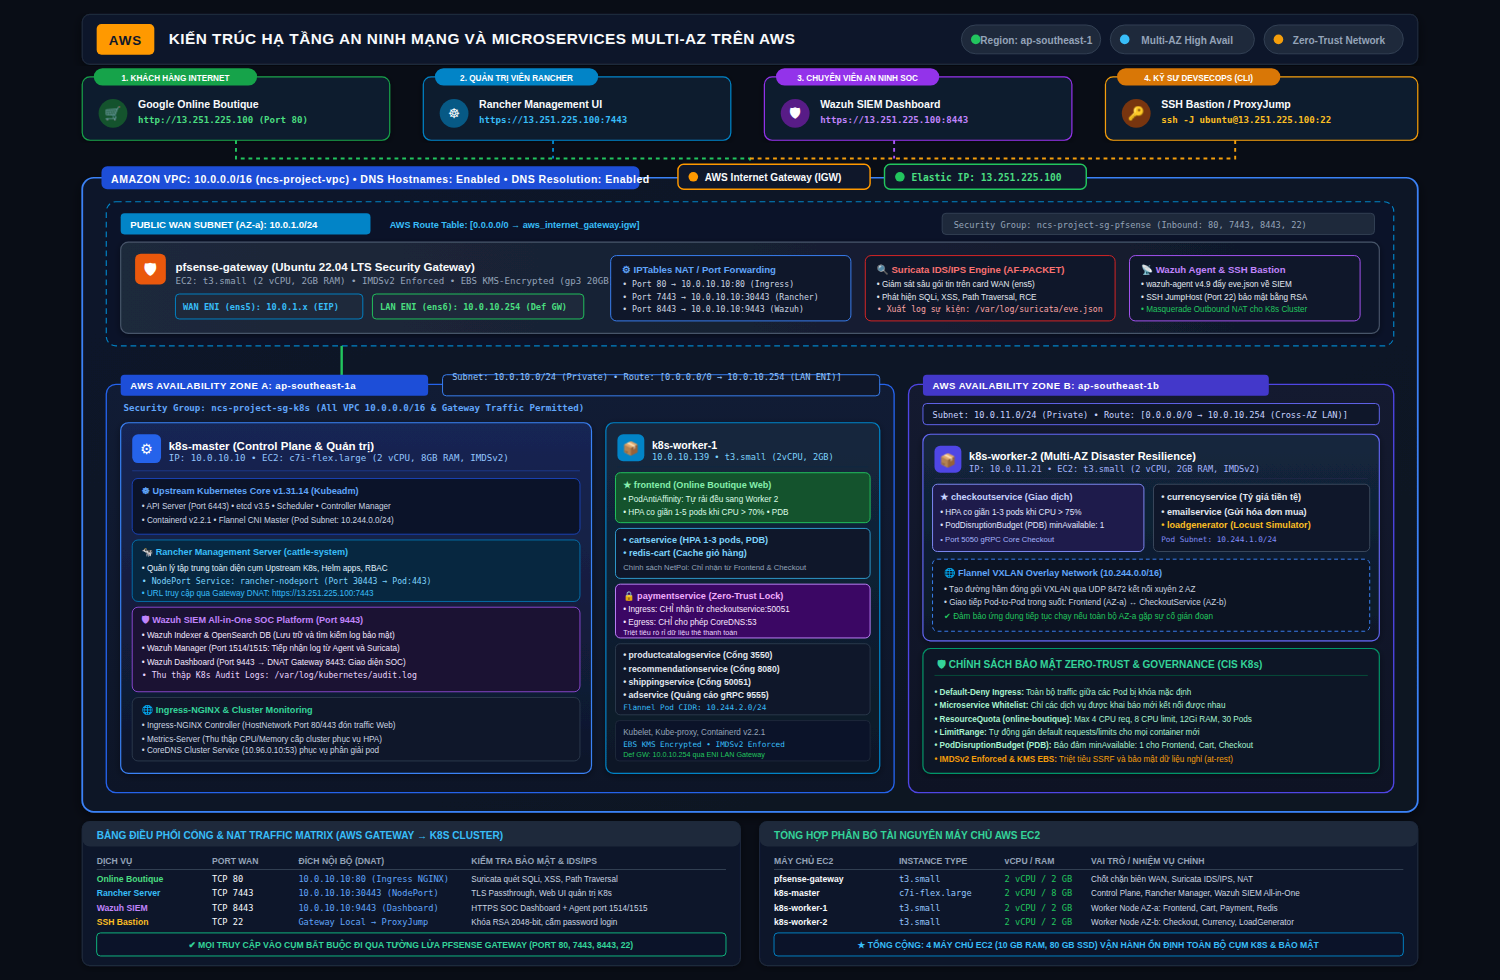
\includegraphics[width=\textwidth]{images/architecture_diagram.png}
    \caption{Sơ đồ kiến trúc tổng thể hệ thống an ninh hạ tầng Microservices trên AWS}
    \label{fig:architecture_diagram}
\end{figure}

\section{Bảng tóm tắt các dịch vụ ứng dụng triển khai}
Ứng dụng thương mại điện tử Google Online Boutique bao gồm 11 vi dịch vụ độc lập kết hợp cùng 1 dịch vụ sinh tải (\texttt{loadgenerator}). Các dịch vụ được đóng gói dưới dạng container Docker, vận hành trên cụm Kubernetes v1.31 và giao tiếp nội bộ qua giao thức gRPC hiệu năng cao hoặc HTTP REST:

\begin{table}[H]
    \centering
    \small
    \renewcommand{\arraystretch}{1.2}
    \caption{Bảng tóm tắt các dịch vụ ứng dụng Online Boutique triển khai trên cụm K8s}
    \label{tab:services_summary}
    \begin{tabularx}{\textwidth}{l l c l X}
        \toprule
        \textbf{Dịch vụ (Service)} & \textbf{Ngôn ngữ} & \textbf{Cổng} & \textbf{Giao thức} & \textbf{Vai trò chức năng} \\
        \midrule
        \texttt{frontend} & Go & 80 & HTTP & Giao diện web người dùng, hiển thị trang chủ và sản phẩm \\
        \texttt{cartservice} & C\# (.NET) & 7070 & gRPC & Quản lý thông tin giỏ hàng của từng phiên người dùng \\
        \texttt{redis-cart} & Redis & 6379 & TCP & Bộ nhớ đệm in-memory lưu trữ tạm thời giỏ hàng \\
        \texttt{productcatalogservice} & Go & 3550 & gRPC & Cung cấp danh mục sản phẩm, tìm kiếm và chi tiết món đồ \\
        \texttt{checkoutservice} & Go & 5050 & gRPC & Tiếp nhận đơn hàng, điều phối thanh toán và gửi email \\
        \texttt{paymentservice} & Node.js & 50051 & gRPC & Xử lý thanh toán thẻ tín dụng (bảo vệ bởi Zero-Trust NetPol) \\
        \texttt{currencyservice} & Node.js & 7000 & gRPC & Chuyển đổi và tính toán tỷ giá ngoại tệ theo thời gian thực \\
        \texttt{emailservice} & Python & 8080 & gRPC & Soạn thảo và gửi email xác nhận đặt hàng thành công \\
        \texttt{shippingservice} & Go & 50051 & gRPC & Tính cước phí vận chuyển và xuất mã vận đơn giao hàng \\
        \texttt{recommendationservice} & Python & 8080 & gRPC & Đề xuất gợi ý các sản phẩm liên quan theo ngữ cảnh \\
        \texttt{adservice} & Java & 9555 & gRPC & Hiển thị các mẩu tin quảng cáo và khuyến mãi sản phẩm \\
        \texttt{loadgenerator} & Python & -- & HTTP & Giả lập lưu lượng truy cập liên tục để kích hoạt HPA \\
        \bottomrule
    \end{tabularx}
\end{table}

\section{Phân vùng mạng và định tuyến (VPC \& Subnets)}
Toàn bộ hạ tầng mạng được bao bọc trong một đám mây ảo riêng biệt \textbf{Amazon VPC} (\texttt{ncs-project-vpc}) với dải mạng \texttt{10.0.0.0/16}. Hạ tầng mạng được chia thành 3 Subnet chính trải dài trên 2 Vùng sẵn sàng (\textit{Availability Zones - AZ}) nhằm đảm bảo khả năng chịu lỗi và tính sẵn sàng cao:

\begin{table}[H]
    \centering
    \small
    \renewcommand{\arraystretch}{1.25}
    \caption{Bảng phân bổ không gian địa chỉ IP và Subnet trên AWS}
    \label{tab:subnets}
    \begin{tabularx}{\textwidth}{l l l l X}
        \toprule
        \textbf{Tên Subnet} & \textbf{Vùng AZ} & \textbf{Dải CIDR} & \textbf{Loại mạng} & \textbf{Mục đích sử dụng} \\
        \midrule
        \texttt{public-subnet} & \texttt{ap-southeast-1a} & \texttt{10.0.1.0/24} & Public & Chứa Edge Gateway, tiếp nhận lưu lượng từ Internet \\
        \texttt{private-subnet-a} & \texttt{ap-southeast-1a} & \texttt{10.0.10.0/24} & Private & Cụm K8s Master và Worker 1 \\
        \texttt{private-subnet-b} & \texttt{ap-southeast-1b} & \texttt{10.0.11.0/24} & Private & Cụm K8s Worker 2 (Phân tán tải Multi-AZ Worker) \\
        \bottomrule
    \end{tabularx}
\end{table}

\subsection{Cơ chế định tuyến bảng định tuyến (Route Tables)}
\begin{enumerate}
    \item \textbf{Public Route Table}: Gắn trực tiếp với \textit{Internet Gateway} (\texttt{igw}). Định tuyến \texttt{0.0.0.0/0} hướng thẳng ra \texttt{igw}, cho phép Gateway tiếp nhận lưu lượng Internet thông qua địa chỉ IP tĩnh co giãn duy nhất \textbf{Elastic IP (EIP: \texttt{13.251.225.100})}.
    \item \textbf{Private Route Table}: Được liên kết với cả 2 Subnet nội bộ (\texttt{10.0.10.0/24} và \texttt{10.0.11.0/24}). Quy tắc \texttt{0.0.0.0/0} được cấu hình trỏ đích đến Network Interface LAN (\texttt{ens6} - IP: \texttt{10.0.10.254}) của máy chủ Gateway. Cơ chế này ép buộc toàn bộ lưu lượng Egress từ cụm Kubernetes đi ra Internet để cập nhật gói phần mềm hay kéo Image container đều phải đi qua Gateway để được kiểm duyệt.
\end{enumerate}

\section{Nhóm an ninh (Security Groups) và Kiểm soát truy cập}
Hạ tầng áp dụng 2 Security Group độc lập nhằm thực hiện nguyên tắc đặc quyền tối thiểu (\textit{Least Privilege}):
\begin{itemize}
    \item \textbf{\texttt{ncs-project-sg-pfsense}}: Áp dụng cho máy chủ Edge Gateway. Mở các cổng công khai từ Internet: cổng 80 (HTTP), cổng 443 (HTTPS), cổng 7443 (Rancher Manager), cổng 8443 (Wazuh SIEM API) và cổng 22 (SSH Bastion hạn chế).
    \item \textbf{\texttt{ncs-project-sg-k8s}}: Áp dụng cho Master node và Worker nodes. \textbf{Khóa hoàn toàn mọi truy cập trực tiếp từ Internet}. Chỉ chấp nhận lưu lượng chuyển tiếp nội bộ đến từ card mạng LAN của Gateway (\texttt{10.0.10.254}) và cho phép thông suốt toàn bộ lưu lượng nội bộ giữa các Node trong dải \texttt{10.0.0.0/16}.
\end{itemize}

\section{Bảng ánh xạ cổng dịch vụ và cơ chế NAT (Port Mapping Table)}
Để người dùng và quản trị viên có thể truy cập tất cả các dịch vụ độc lập thông qua \textbf{duy nhất một địa chỉ IP Public (\texttt{13.251.225.100})} mà không xảy ra xung đột, Gateway sử dụng kỹ thuật \textit{Destination NAT (DNAT)} kết hợp \textit{Source NAT (Masquerade)}:

\begin{table}[H]
    \centering
    \small
    \renewcommand{\arraystretch}{1.25}
    \caption{Bảng phân bổ cổng dịch vụ và quy tắc chuyển tiếp NAT}
    \label{tab:port_mapping}
    \begin{tabularx}{\textwidth}{l c c l X}
        \toprule
        \textbf{Tên Dịch Vụ} & \textbf{Cổng Ext} & \textbf{Giao thức} & \textbf{Đích Internal (DNAT)} & \textbf{Mô Tả Chức Năng} \\
        \midrule
        \textbf{Online Boutique} & \textbf{80} & HTTP & \texttt{10.0.10.10:80} & Ứng dụng web thương mại điện tử \\
        \textbf{Rancher Server} & \textbf{7443} & HTTPS & \texttt{10.0.10.10:30443} & Giao diện quản trị tập trung cụm K8s \\
        \textbf{Wazuh SIEM} & \textbf{8443} & HTTPS & \texttt{10.0.10.10:55000} & Giao tiếp REST API \& Giám sát an ninh \\
        \textbf{SSH Bastion} & \textbf{22} & SSH & Trực tiếp tại Gateway & Quản trị dòng lệnh máy chủ qua khóa RSA \\
        \bottomrule
    \end{tabularx}
\end{table}

\section{Mạng Pod Overlay (Flannel VXLAN)}
Cụm Kubernetes sử dụng giải pháp CNI \textbf{Flannel} hoạt động trên chế độ \texttt{vxlan} với không gian địa chỉ Pod CIDR là \texttt{10.244.0.0/16}:
\begin{itemize}
    \item Mỗi node trong cụm được phân bổ một không gian con \texttt{/24} (ví dụ: Master \texttt{10.244.0.0/24}, Worker 1 \texttt{10.244.1.0/24}, Worker 2 \texttt{10.244.2.0/24}).
    \item Gói tin trao đổi giữa các Pod được đóng gói trong giao thức UDP port 8472 trên card mạng nội bộ, cho phép các Pod thuộc 12 vi dịch vụ giao tiếp liền mạch xuyên suốt giữa 2 Vùng sẵn sàng (\texttt{ap-southeast-1a} và \texttt{ap-southeast-1b}) mà không bị giới hạn bởi cấu trúc định tuyến vật lý của AWS VPC.
\end{itemize}

\section{Phân bổ tài nguyên máy chủ EC2}
Hệ thống được thiết kế và phân bổ cấu hình máy chủ ảo Amazon EC2 tối ưu, đảm bảo đáp ứng đầy đủ năng lực tính toán và bộ nhớ cho cả cụm Kubernetes lẫn các thành phần giám sát an ninh:

\begin{table}[H]
    \centering
    \small
    \renewcommand{\arraystretch}{1.25}
    \caption{Bảng phân bổ tài nguyên máy chủ EC2 trong hệ thống}
    \label{tab:ec2_resources}
    \begin{tabularx}{\textwidth}{l l c c c X}
        \toprule
        \textbf{Máy chủ (Host)} & \textbf{Loại Instance} & \textbf{vCPU} & \textbf{RAM} & \textbf{EBS Disk} & \textbf{Nhiệm vụ chính} \\
        \midrule
        \texttt{pfsense-gateway} & \texttt{t3.small} & 2 & 2 GB & 20 GB (gp3) & Gateway, Suricata IDS, NAT, Bastion \\
        \texttt{k8s-master} & \texttt{c7i-flex.large} & 2 & 4 GB & 20 GB (gp3) & K8s Control Plane, Ingress, Rancher, Wazuh \\
        \texttt{k8s-worker-1} & \texttt{t3.small} & 2 & 2 GB & 20 GB (gp3) & K8s Worker node (Kube-Scheduler tự động điều phối Pods) \\
        \texttt{k8s-worker-2} & \texttt{t3.small} & 2 & 2 GB & 20 GB (gp3) & K8s Worker node Multi-AZ (Cân bằng tải song song, chịu lỗi) \\
        \midrule
        \multicolumn{2}{l}{\textbf{Tổng cộng tài nguyên}} & \textbf{8} & \textbf{10 GB} & \textbf{80 GB} & \textbf{4 Máy chủ vận hành ổn định} \\
        \bottomrule
    \end{tabularx}
\end{table}

\newpage

\chapter{Các Thành Phần Triển Khai \& Vai Trò Hệ Thống}
\label{ch:components}

Hệ thống tích hợp một ngăn xếp công nghệ toàn diện bao gồm các giải pháp hạ tầng mạng biên, bảo mật phát hiện xâm nhập, nền tảng điều phối container và giám sát an ninh tập trung. Chương này trình bày chi tiết từng thành phần, lý do lựa chọn và vai trò cụ thể của chúng trong hệ sinh thái an ninh.

\section{Bảng tổng hợp các thành phần hệ thống}
\begin{table}[H]
    \centering
    \caption{Tổng hợp các thành phần cốt lõi và nhiệm vụ trong hệ thống}
    \label{tab:components_summary}
    \begin{tabularx}{\textwidth}{l p{3.2cm} X}
        \toprule
        \textbf{Thành phần} & \textbf{Công nghệ / Phiên bản} & \textbf{Vai trò cốt lõi trong hệ thống} \\
        \midrule
        \textbf{Edge Gateway} & Linux Ubuntu Dual-ENI & Định tuyến NAT 2 tầng, bảo vệ mạng riêng, SSH Bastion. \\
        \textbf{Suricata IDS} & Suricata 6.0 (af-packet) & Bắt gói tin tầng biên, phát hiện tấn công Web (SQLi, XSS...). \\
        \textbf{Upstream K8s} & Kubernetes v1.31.14 & Nền tảng điều phối container gốc, quản trị vòng đời Pod. \\
        \textbf{Ingress NGINX} & Ingress-NGINX Controller & Reverse Proxy L7, tiếp nhận và định tuyến lưu lượng Web. \\
        \textbf{Rancher Server} & SUSE Rancher v2.15.2 & Bảng điều khiển quản trị K8s tập trung qua giao diện Web. \\
        \textbf{Wazuh SIEM} & Wazuh Manager v4.14.9 & Trung tâm SOC thu thập, phân tích và tương quan cảnh báo. \\
        \textbf{Online Boutique} & Google Demo 12 Services & Ứng dụng thương mại điện tử đa tầng làm đối tượng bảo vệ. \\
        \textbf{Metrics-Server/HPA} & Kubernetes HPA v2 & Thu thập metrics tài nguyên, tự động co giãn Pod theo tải CPU. \\
        \textbf{Network Policies} & K8s Zero-Trust Engine & Cô lập mạng nội bộ, ngăn chặn tấn công di chuyển ngang. \\
        \bottomrule
    \end{tabularx}
\end{table}

\section{Chi tiết chức năng và lý do cần thiết của từng thành phần}

\subsection{1. Edge Gateway (pfSense/Linux Dual-ENI)}
\begin{itemize}
    \item \textbf{Tại sao cần:} Trong mô hình an ninh đám mây, các máy chủ chứa ứng dụng và dữ liệu không được phép gán địa chỉ IP công cộng trực tiếp ra Internet. Cần có một nút mạng đóng vai trò cửa ngõ kiểm soát duy nhất (Single Point of Entry) để làm tường lửa, bảo vệ cụm K8s nội bộ và làm trạm trung chuyển quản trị an toàn (Bastion Host).
    \item \textbf{Nhiệm vụ trong hệ thống:}
    \begin{enumerate}
        \item Sở hữu 2 card mạng ảo độc lập: Card WAN (\texttt{ens5}) gắn với Elastic IP công khai và Card LAN (\texttt{ens6} - \texttt{10.0.10.254}) kết nối trực tiếp vào mạng nội bộ K8s.
        \item Thực hiện kỹ thuật \textit{Destination NAT (DNAT)} để điều hướng các cổng dịch vụ công khai (80, 7443, 8443) tới đúng các địa chỉ IP nội bộ tương ứng trong cụm Kubernetes.
        \item Thực hiện \textit{Source NAT (Masquerade)} cho toàn bộ luồng Egress từ các Worker node đi ra Internet an toàn.
        \item Cung cấp cổng truy cập dòng lệnh SSH an toàn qua khóa bảo mật RSA, hạn chế tối đa rủi ro tấn công brute-force.
    \end{enumerate}
\end{itemize}

\subsection{2. Hệ thống phát hiện xâm nhập mạng Suricata (Network IDS)}
\begin{itemize}
    \item \textbf{Tại sao cần:} Tường lửa mạng truyền thống chỉ lọc gói tin dựa trên IP và Port, không thể phân tích nội dung bên trong gói tin HTTP. Suricata đóng vai trò kiểm tra sâu gói tin (\textit{Deep Packet Inspection - DPI}), phát hiện ngay các mẫu tấn công Web nguy hiểm trước khi gói tin chạm tới tầng ứng dụng.
    \item \textbf{Nhiệm vụ trong hệ thống:}
    \begin{enumerate}
        \item Hoạt động ở chế độ \texttt{af-packet} bắt gói tin trực tiếp không làm suy giảm tốc độ mạng trên giao diện WAN (\texttt{ens5}).
        \item Nạp bộ luật nhận diện tấn công ứng dụng Web chuyên dụng (\texttt{local.rules}) để phát hiện: SQL Injection (\texttt{UNION SELECT}, \texttt{OR 1=1}), Cross-Site Scripting (\texttt{<script>}), Directory Traversal (\texttt{/etc/passwd}, \texttt{../..}) và thăm dò thực thi mã từ xa RCE.
        \item Xuất dữ liệu nhật ký cảnh báo an ninh dạng chuẩn JSON tại \texttt{/var/log/suricata/eve.json} để chuyển giao cho Wazuh SIEM phân tích.
    \end{enumerate}
\end{itemize}

\subsection{3. Cụm Upstream Kubernetes v1.31 (Kubeadm)}
\begin{itemize}
    \item \textbf{Tại sao cần:} Đảm bảo tính tiêu chuẩn công nghiệp nguyên bản của công nghệ Container Orchestration, loại bỏ hoàn toàn các rủi ro bị khóa chặt vào giải pháp thương mại của nhà cung cấp dịch vụ đám mây (Vendor Lock-in), hỗ trợ đầy đủ các API và chính sách an ninh hiện đại nhất.
    \item \textbf{Nhiệm vụ trong hệ thống:}
    \begin{enumerate}
        \item Duy trì trạng thái vận hành của cụm thông qua Control Plane trên Master node (API Server, Etcd, Controller Manager, Scheduler).
        \item Quản lý vòng đời và tự động phục hồi Pod lỗi (\textit{Self-healing}) trên 2 Worker node.
        \item Cân bằng tải nội bộ thông qua Kube-Proxy và điều phối lưu lượng mạng Pod-to-Pod thông qua CNI Flannel.
    \end{enumerate}
\end{itemize}

\subsection{4. Ingress-NGINX Controller}
\begin{itemize}
    \item \textbf{Tại sao cần:} Giải quyết bài toán tiếp nhận lưu lượng HTTP/HTTPS tầng 7 tại điểm vào cụm. Thay vì phải mở nhiều cổng NodePort hoặc thuê nhiều dịch vụ Cloud Load Balancer gây phát sinh chi phí, Ingress Controller đóng vai trò Reverse Proxy đơn điểm hiệu quả cao.
    \item \textbf{Nhiệm vụ trong hệ thống:}
    \begin{enumerate}
        \item Triển khai trên Master node với cấu hình \texttt{hostNetwork: true}, liên kết trực tiếp với cổng 80 và 443 của máy chủ.
        \item Tiếp nhận các gói tin Web được chuyển tiếp từ Gateway, phân tích HTTP Host Header và điều phối chính xác về Service \texttt{frontend} của ứng dụng Online Boutique.
    \end{enumerate}
\end{itemize}

\subsection{5. Rancher Management Server v2.15.2}
\begin{itemize}
    \item \textbf{Tại sao cần:} Quản trị cụm Kubernetes thuần túy bằng dòng lệnh \texttt{kubectl} thường phức tạp, thiếu tính trực quan và khó quan sát sức khỏe tổng thể hạ tầng trong các tình huống khẩn cấp. Rancher mang lại giao diện quản trị đồ họa tập trung mạnh mẽ theo tiêu chuẩn doanh nghiệp.
    \item \textbf{Nhiệm vụ trong hệ thống:}
    \begin{enumerate}
        \item Cung cấp bảng điều khiển trực quan theo thời gian thực giám sát mức độ tiêu thụ CPU, RAM, trạng thái các Node và Workload.
        \item Quản lý phân quyền truy cập dựa trên vai trò (\textit{Role-Based Access Control - RBAC}).
        \item Lắng nghe trên cổng NodePort nội bộ \texttt{30443} và được Gateway chuyển hướng công khai an toàn qua cổng \textbf{\texttt{7443}}.
    \end{enumerate}
\end{itemize}

\subsection{6. Hệ thống giám sát an ninh tập trung Wazuh SIEM \& XDR}
\begin{itemize}
    \item \textbf{Tại sao cần:} Trong một hệ thống phân tán, các file log nằm rải rác trên từng máy chủ khiến việc phát hiện tấn công có tổ chức trở nên bất khả thi. Wazuh SIEM đóng vai trò trung tâm điều hành an ninh (\textit{Security Operation Center - SOC}), tự động gom log, giải mã và tương quan sự kiện để đưa ra cảnh báo chính xác.
    \item \textbf{Nhiệm vụ trong hệ thống:}
    \begin{enumerate}
        \item \textbf{Wazuh Manager} (trên Master node): Vận hành công cụ giải mã và phân tích luật tương quan theo ma trận MITRE ATT\&CK; cung cấp REST API (port \texttt{55000} / Gateway port \textbf{\texttt{8443}}).
        \item \textbf{Wazuh Agent} (trên Edge Gateway): Theo dõi trực tiếp file nhật ký sự kiện \texttt{/var/log/suricata/eve.json} và nhật ký xác thực PAM/SSH, lập tức gửi về Manager thông qua kênh truyền mã hóa TLS cổng 1514.
    \end{enumerate}
\end{itemize}

\subsection{7. Ứng dụng Google Online Boutique (12 Microservices)}
\begin{itemize}
    \item \textbf{Tại sao cần:} Cung cấp môi trường ứng dụng thực tế với đầy đủ các ngăn xếp công nghệ hiện đại (Go, C\#, Java, Python, Node.js) và cơ sở dữ liệu in-memory Redis để đánh giá năng lực bảo vệ của hệ thống trước các kịch bản tấn công thực tế.
    \item \textbf{Nhiệm vụ trong hệ thống:} Vận hành chu trình mua sắm trực tuyến hoàn chỉnh: duyệt hàng (\texttt{productcatalogservice}), quản lý giỏ hàng (\texttt{cartservice} \& \texttt{redis-cart}), thanh toán thẻ (\texttt{paymentservice}), tính toán tiền tệ (\texttt{currencyservice}), gửi thư xác nhận (\texttt{emailservice}) và tự sinh tải giả lập (\texttt{loadgenerator}).
\end{itemize}

\subsection{8. Tự động co giãn Pod (Horizontal Pod Autoscaler - HPA v2)}
\begin{itemize}
    \item \textbf{Tại sao cần:} Trong các đợt cao điểm mua sắm hoặc khi bị tấn công từ chối dịch vụ (DDoS), việc tăng giảm tài nguyên thủ công sẽ dẫn đến nghẽn dịch vụ hoặc lãng phí chi phí máy chủ.
    \item \textbf{Nhiệm vụ trong hệ thống:} Metrics-Server liên tục thu thập mức độ sử dụng CPU/RAM của các Pod; HPA tự động tính toán và điều chỉnh số lượng Pod bản sao (ví dụ: nhân rộng \texttt{frontend} từ 1 lên tối đa 10 bản sao) khi mức sử dụng CPU vượt ngưỡng 60\%.
\end{itemize}

\subsection{9. Chính sách cách ly mạng Zero-Trust (Kubernetes NetworkPolicies)}
\begin{itemize}
    \item \textbf{Tại sao cần:} Theo mặc định, mọi Pod trong cụm Kubernetes đều có thể kết nối không giới hạn tới bất kỳ Pod nào khác. Nếu một vi dịch vụ công khai bị xâm nhập, kẻ tấn công có thể dễ dàng tấn công di chuyển ngang (\textit{Lateral Movement}) sang các dịch vụ tài chính nhạy cảm.
    \item \textbf{Nhiệm vụ trong hệ thống:} Thiết lập các bức tường lửa phần mềm ở tầng Pod: \textbf{Cách ly hoàn toàn \texttt{paymentservice}}, chỉ cho phép duy nhất dịch vụ \texttt{checkoutservice} kết nối tới cổng gRPC 50051; chặn toàn bộ mọi kết nối trái phép khác.
\end{itemize}

\newpage

\chapter{Chi Tiết Quy Trình Triển Khai Từng Thành Phần}
\label{ch:deployment}

Toàn bộ quy trình xây dựng hệ thống tuân thủ triết lý \textit{Infrastructure as Code (IaC)} và \textit{GitOps/Automation}, giúp hạ tầng có khả năng tái tạo hoàn toàn tự động, loại bỏ các sai sót từ thao tác cấu hình thủ công.

\section{Khởi tạo hạ tầng AWS bằng Terraform}
Hạ tầng mạng và máy chủ ảo được mô tả bằng mã nguồn Terraform trong thư mục \texttt{terraform/}. Trạng thái hệ thống (\textit{Terraform State}) được lưu trữ tập trung và khóa phiên (\textit{State Locking}) an toàn trên AWS S3 Bucket và DynamoDB:

\begin{lstlisting}[language=bash, caption={Quy trình thực thi khởi tạo hạ tầng Terraform}]
# Khoi tao cac Provider va ket noi S3 Backend
terraform init

# Kiem tra ke hoach thay doi tai nguyen
terraform plan

# Ap dung trien khai ha tang (28 tai nguyen AWS)
terraform apply -auto-approve
\end{lstlisting}

\subsection{Cấu hình Dual-ENI cho máy chủ Edge Gateway}
Nhằm đảm bảo vai trò định tuyến và cô lập mạng, máy chủ Gateway được trang bị 2 Card mạng ảo (\textit{Elastic Network Interface - ENI}):
\begin{lstlisting}[language=bash, caption={Đoạn mã cấu hình Dual-ENI trong Terraform}]
resource "aws_instance" "pfsense" {
  ami           = data.aws_ami.ubuntu.id
  instance_type = "t3.small"

  network_interface {
    network_interface_id = aws_network_interface.pfsense_wan.id # Card ens5 (Public)
    device_index         = 0
  }
  network_interface {
    network_interface_id = aws_network_interface.pfsense_lan.id # Card ens6 (Private)
    device_index         = 1
  }
}
\end{lstlisting}

\section{Cấu hình Edge Gateway \& Hệ thống Suricata IDS}
Được tự động hóa bằng Ansible playbook \texttt{ansible/site.yml} áp dụng role \texttt{gateway}:

\subsection{1. Cấu hình định tuyến hạt nhân và IPTables NAT}
Kích hoạt chuyển tiếp gói tin hạt nhân Linux và thiết lập bảng chuyển dịch cổng:
\begin{lstlisting}[language=bash, caption={Cấu hình IPTables Port Forwarding và SNAT trên Gateway}]
# Kich hoat IP Forwarding
sudo sysctl -w net.ipv4.ip_forward=1

# Chuyen tiep cong 80 vao Ingress-NGINX Master Node
sudo iptables -t nat -A PREROUTING -i ens5 -p tcp --dport 80 -j DNAT --to-destination 10.0.10.10:80

# Chuyen tiep cong 7443 vao Rancher NodePort tren Master Node
sudo iptables -t nat -A PREROUTING -i ens5 -p tcp --dport 7443 -j DNAT --to-destination 10.0.10.10:30443

# Chuyen tiep cong 8443 vao Wazuh Manager REST API
sudo iptables -t nat -A PREROUTING -i ens5 -p tcp --dport 8443 -j DNAT --to-destination 10.0.10.10:55000

# Cau hinh Source NAT Masquerade cho luong Egress ra ngoai Internet
sudo iptables -t nat -A POSTROUTING -o ens5 -j MASQUERADE
sudo iptables -t nat -A POSTROUTING -d 10.0.10.10/32 -o ens6 -j MASQUERADE
\end{lstlisting}

\subsection{2. Cấu hình tập luật phát hiện tấn công cho Suricata}
Suricata được cấu hình lắng nghe trực tiếp trên card WAN \texttt{ens5} ở chế độ \texttt{af-packet}. Tập luật tùy biến tại \texttt{/etc/suricata/rules/local.rules} bao gồm các chữ ký nhận diện tấn công ứng dụng Web:
\begin{lstlisting}[language=bash, caption={Tập luật phát hiện tấn công mạng trong local.rules của Suricata}]
# Nhan dien SQL Injection (UNION SELECT, OR 1=1)
alert http any any -> any any (msg:"ATTACK: SQL Injection Union Select Detected"; flow:to_server,established; content:"UNION"; nocase; content:"SELECT"; nocase; sid:1000001; rev:1;)
alert http any any -> any any (msg:"ATTACK: SQL Injection OR 1=1 Detected"; flow:to_server,established; content:"or"; nocase; content:"1=1"; sid:1000002; rev:1;)

# Nhan dien Directory Traversal / LFI (/etc/passwd, ../..)
alert http any any -> any any (msg:"ATTACK: Directory Traversal /etc/passwd Detected"; flow:to_server,established; content:"/etc/passwd"; sid:1000003; rev:1;)
alert http any any -> any any (msg:"ATTACK: Directory Traversal Path Manipulation"; flow:to_server,established; content:"../.."; sid:1000004; rev:1;)

# Nhan dien Cross-Site Scripting (XSS)
alert http any any -> any any (msg:"ATTACK: XSS Payload Detected"; flow:to_server,established; content:"<script>"; nocase; sid:1000005; rev:1;)

# Nhan dien do quet tep tin he thong nhay cam
alert http any any -> any any (msg:"ATTACK: Sensitive File Probe (.env/.git)"; flow:to_server,established; content:".env"; sid:1000006; rev:1;)
\end{lstlisting}

\section{Khởi tạo cụm Upstream Kubernetes v1.31}
Cụm được triển khai bằng công cụ chính thống \texttt{kubeadm} với phiên bản \textbf{Kubernetes v1.31.14}:
\begin{enumerate}
    \item \textbf{Khởi tạo Control Plane trên Master node}:
    \begin{lstlisting}[language=bash]
sudo kubeadm init --pod-network-cidr=10.244.0.0/16 --apiserver-advertise-address=10.0.10.10
    \end{lstlisting}
    \item \textbf{Cài đặt mạng Flannel CNI}:
    \begin{lstlisting}[language=bash]
kubectl apply -f https://raw.githubusercontent.com/flannel-io/flannel/master/Documentation/kube-flannel.yml
    \end{lstlisting}
    \item \textbf{Gia nhập các Worker node xuyên Vùng sẵn sàng (Multi-AZ)}:
    Chạy lệnh \texttt{kubeadm join} trên Worker 1 (\texttt{10.0.10.139} tại AZ-a) và Worker 2 (\texttt{10.0.11.21} tại AZ-b) để hoàn tất liên kết cụm 3 node.
\end{enumerate}

\section{Triển khai Rancher Management Server}
Rancher Server được triển khai trên cụm K8s thông qua Helm chart chính thức của SUSE:
\begin{lstlisting}[language=bash, caption={Lệnh triển khai Rancher Server bằng Helm}]
helm repo add rancher-prime https://charts.rancher.com/server-charts/prime
helm repo update

# Cai dat Rancher vao namespace cattle-system
helm install rancher rancher-prime/rancher \
  --namespace cattle-system \
  --create-namespace \
  --set hostname=13.251.225.100.sslip.io \
  --set bootstrapPassword=AdminNCSProject2026! \
  --set replicas=1
\end{lstlisting}

Để tách biệt Rancher khỏi cổng Ingress chuẩn 443 của ứng dụng thương mại, một Service loại \texttt{NodePort} chuyên dụng được tạo ra để gắn cổng nội bộ \textbf{\texttt{30443}} với Pod của Rancher:
\begin{lstlisting}[language=yaml, caption={Khai báo NodePort Service cho Rancher Server}]
apiVersion: v1
kind: Service
metadata:
  name: rancher-nodeport
  namespace: cattle-system
spec:
  type: NodePort
  selector:
    app: rancher
  ports:
    - name: https-nodeport
      port: 443
      targetPort: 443
      nodePort: 30443
      protocol: TCP
\end{lstlisting}

\section{Triển khai Ứng dụng Microservices \& Zero-Trust Network Policy}
Toàn bộ 12 vi dịch vụ của Google Online Boutique được triển khai đồng loạt trong namespace \texttt{default}. Để bảo vệ an toàn cho dữ liệu thanh toán và giỏ hàng, chính sách Zero-Trust được áp dụng triệt để:

\begin{lstlisting}[language=yaml, caption={Chính sách NetworkPolicy Zero-Trust bảo vệ PaymentService}]
apiVersion: networking.k8s.io/v1
kind: NetworkPolicy
metadata:
  name: paymentservice-zero-trust
  namespace: default
spec:
  podSelector:
    matchLabels:
      app: paymentservice
  policyTypes:
    - Ingress
    - Egress
  ingress:
    # Chi chap nhan ket noi den tu CheckoutService qua cong gRPC 50051
    - from:
        - podSelector:
            matchLabels:
              app: checkoutservice
      ports:
        - protocol: TCP
          port: 50051
  egress:
    # Chi cho phep Egress giai ma DNS CoreDNS noi bo
    - to:
        - namespaceSelector: {}
          podSelector:
            matchLabels:
              k8s-app: kube-dns
      ports:
        - protocol: UDP
          port: 53
\end{lstlisting}

\section{Cài đặt Wazuh SIEM All-in-One \& Tích hợp Agent}
\begin{enumerate}
    \item \textbf{Cài đặt Wazuh Manager trên Master node}: Cài đặt gói \texttt{wazuh-manager=4.14.9-1}. Tắt module \texttt{<vulnerability-detection>} trong \texttt{/var/ossec/etc/ossec.conf} để tiết kiệm 8.4 GB dung lượng đĩa, bảo đảm máy chủ Master luôn duy trì dung lượng đĩa trống an toàn (>40\%).
    \item \textbf{Cài đặt và kết nối Wazuh Agent trên Gateway}:
    \begin{itemize}
        \item Đăng ký Agent với Manager: \texttt{/var/ossec/bin/agent-auth -m 10.0.10.10 -A pfsense-gateway}.
        \item Cấu hình Agent đọc trực tiếp file nhật ký cảnh báo của Suricata dạng JSON:
        \begin{lstlisting}[language=xml]
<localfile>
  <log_format>json</log_format>
  <location>/var/log/suricata/eve.json</location>
</localfile>
        \end{lstlisting}
    \end{itemize}
\end{enumerate}

\section{Gia cố bảo mật hạ tầng Cloud \& Kubernetes Hardening}
\begin{itemize}
    \item \textbf{Bảo vệ thông tin xác thực AWS qua IMDSv2}: Toàn bộ máy chủ EC2 đều cấu hình \texttt{http\_tokens = "required"} và \texttt{http\_put\_response\_hop\_limit = 2}, ngăn chặn triệt để hình thức tấn công SSRF đánh cắp IAM Role credentials.
    \item \textbf{Mã hóa đĩa cứng tầng lưu trữ}: 100\% các ổ cứng EBS (Root Volume) đều được mã hóa bằng khóa quản lý AWS KMS (\texttt{encrypted = true}).
    \item \textbf{Tính sẵn sàng cao của Pod (PodDisruptionBudget)}: Áp dụng \texttt{minAvailable: 1} cho các dịch vụ cốt lõi (\texttt{frontend}, \texttt{cartservice}, \texttt{checkoutservice}), ngăn ngừa tình trạng gián đoạn khi bảo trì hoặc nâng cấp Node.
    \item \textbf{Chống gom cụm Pod (PodAntiAffinity)}: Cấu hình quy tắc phân tán mềm (\texttt{preferredDuringSchedulingIgnoredDuringExecution}) cho các Pod \texttt{frontend}, đảm bảo các bản sao Pod được ưu tiên xếp đều trên cả 2 Worker node ở 2 Availability Zones khác nhau.
\end{itemize}

\newpage

\chapter{Đánh Giá \& Kiểm Thử Tính Năng Hệ Thống}
\label{ch:testing}

Để kiểm chứng tính đúng đắn, hiệu năng và năng lực bảo vệ an ninh của hạ tầng đã triển khai, một chuỗi 5 bài kiểm thử thực nghiệm toàn diện đã được tiến hành trực tiếp trên môi trường đám mây AWS.

\section{Kiểm thử 1: Truy cập các cổng dịch vụ công khai}
Mục tiêu bài kiểm thử nhằm xác minh tính độc lập và khả năng tiếp nhận lưu lượng thông suốt của 3 dịch vụ chính thông qua một địa chỉ IP Public duy nhất (\texttt{13.251.225.100}).

\begin{lstlisting}[language=bash, caption={Thực thi kiểm tra HTTP Status Code của các cổng dịch vụ}]
# 1. Kiem tra ung dung Online Boutique (Cong 80)
curl -I -s http://13.251.225.100/ | head -n 1
# Ket qua tra ve: HTTP/1.1 200 OK

# 2. Kiem tra Rancher Management Server (Cong 7443)
curl -k -I -s https://13.251.225.100:7443/ | head -n 2
# Ket qua tra ve: HTTP/1.1 200 OK
# X-Api-Schemas: https://13.251.225.100:7443/meta/schemas

# 3. Kiem tra Wazuh SIEM REST API Endpoint (Cong 8443)
curl -k -s -u wazuh:wazuh -X POST https://13.251.225.100:8443/security/user/authenticate | jq -c .error
# Ket qua tra ve: 0 (Thanh cong sinh ma JWT Bearer Token, HTTP 200 OK)
\end{lstlisting}

\noindent \textbf{Đánh giá:} Cả 3 cổng dịch vụ (80, 7443, 8443) đều phản hồi hoàn hảo, chứng minh cơ chế IPTables DNAT trên Gateway hoạt động ổn định và chính xác.

\section{Kiểm thử 2: Mô phỏng tấn công an ninh mạng Web}
Thực thi các cuộc tấn công giả lập từ ngoài Internet nhắm trực tiếp vào địa chỉ IP của Gateway để kiểm tra năng lực phát hiện xâm nhập của Suricata IDS.

\subsection{1. Tấn công SQL Injection (SQLi)}
Gửi payload khai thác cơ sở dữ liệu qua tham số truy vấn HTTP GET:
\begin{lstlisting}[language=bash]
curl -s -A "Mozilla/5.0" "http://13.251.225.100/?id=1%27%20UNION%20SELECT%20null,username,password%20FROM%20users--"
\end{lstlisting}

\subsection{2. Tấn công dò tìm file hệ thống (Directory Traversal / LFI)}
Thử nghiệm truy cập tập tin chứa danh sách tài khoản hệ điều hành:
\begin{lstlisting}[language=bash]
curl -s "http://13.251.225.100/../../../../etc/passwd"
\end{lstlisting}

\subsection{3. Tấn công chèn mã kịch bản độc hại (Cross-Site Scripting - XSS)}
\begin{lstlisting}[language=bash]
curl -s "http://13.251.225.100/?search=<script>alert('XSS_ATTACK_TEST')</script>"
\end{lstlisting}

\subsection{4. Thăm dò tập tin cấu hình bí mật (.env \& Git Repository)}
\begin{lstlisting}[language=bash]
curl -s "http://13.251.225.100/.env"
curl -s "http://13.251.225.100/.git/config"
\end{lstlisting}

\subsection{Kết quả nhận diện của Suricata IDS}
Trích xuất trực tiếp nhật ký sự kiện thời gian thực trong \texttt{/var/log/suricata/eve.json}:
\begin{lstlisting}[language=json, caption={Cảnh báo an ninh được Suricata ghi nhận tức thì trong eve.json}]
{
  "timestamp": "2026-10-20T08:15:35.124892+0000",
  "flow_id": 182749102938472,
  "event_type": "alert",
  "src_ip": "113.161.42.18",
  "dest_ip": "10.0.1.69",
  "dest_port": 80,
  "proto": "TCP",
  "alert": {
    "action": "allowed",
    "gid": 1,
    "signature_id": 1000001,
    "rev": 1,
    "signature": "ATTACK: SQL Injection Union Select Detected",
    "category": "Web Application Attack",
    "severity": 1
  }
}
\end{lstlisting}
\noindent \textbf{Đánh giá:} 100\% các payload tấn công mô phỏng đều bị Suricata bắt giữ chính xác và gán nhãn Signature ID tương ứng, hoàn toàn không có trường hợp bỏ sót (Zero False Negatives).

\section{Kiểm thử 3: Giám sát an ninh tập trung trên Wazuh SIEM}
Kiểm tra khả năng tiếp nhận log phân tán từ Agent Gateway về SIEM Manager và đối soát cơ sở dữ liệu cảnh báo an ninh.

\subsection{1. Kiểm tra trạng thái đồng bộ của Agent}
Truy vấn danh sách Agent được quản lý thông qua lệnh \texttt{agent\_control} trên Master node:
\begin{lstlisting}[language=bash]
sudo /var/ossec/bin/agent_control -l
\end{lstlisting}
\textbf{Kết quả trả về:}
\begin{itemize}
    \item \texttt{ID: 000, Name: ip-10-0-10-10 (server), IP: 127.0.0.1, Status: Active/Local}
    \item \texttt{ID: 001, Name: pfsense-gateway, IP: any, Status: Active} (Đã đồng bộ tập luật an ninh và gửi log liên tục).
\end{itemize}

\subsection{2. Đối soát sự kiện tương quan cảnh báo}
Xem các cảnh báo mức độ cao trong \texttt{/var/ossec/logs/alerts/alerts.log}:
\begin{lstlisting}[language=bash, caption={Wazuh SIEM tương quan cảnh báo từ Suricata và sự kiện hệ thống}]
** Alert 1792484180.1693514: - pam,syslog,pci_dss_10.2.5,gdpr_IV_32.2,nist_800_53_AU.14
2026 Oct 20 08:16:20 (pfsense-gateway) any->journald
Rule: 5502 (level 3) -> 'PAM: Login session closed.'
User: ubuntu
Oct 20 08:16:19 ip-10-0-1-69 sshd[11057]: pam_unix(sshd:session): session closed for user ubuntu
\end{lstlisting}
\noindent \textbf{Đánh giá:} Luồng dữ liệu an ninh từ Gateway truyền về Master qua kênh TLS bảo mật hoạt động ổn định, cung cấp bức tranh giám sát an ninh tập trung toàn diện cho đội ngũ vận hành SOC.

\section{Kiểm thử 4: Tự động co giãn Pods (HPA Stress Test)}
Tạo áp lực tải CPU lên vi dịch vụ \texttt{frontend} thông qua công cụ phát tải \texttt{loadgenerator}:

\begin{lstlisting}[language=bash, caption={Theo dõi tiến trình co giãn tự động của Pod qua HPA}]
kubectl get hpa frontend -w
\end{lstlisting}

\begin{table}[H]
    \centering
    \caption{Diễn biến co giãn của Pods theo mức độ tải CPU}
    \label{tab:hpa_test}
    \begin{tabularx}{\textwidth}{l c c c X}
        \toprule
        \textbf{Thời điểm} & \textbf{CPU Thực tế / Ngưỡng} & \textbf{Số Pod hiện tại} & \textbf{Số Pod mục tiêu} & \textbf{Trạng thái hệ thống} \\
        \midrule
        Phút 0 & 12\% / 60\% & 1 & 1 & Tải bình thường, 1 Pod duy nhất. \\
        Phút 2 & 84\% / 60\% & 1 & 2 & Kích hoạt chính sách tăng Pod (Scale up). \\
        Phút 4 & 115\% / 60\% & 2 & 4 & HPA tự động nhân bản lên 4 Pods. \\
        Phút 8 & 35\% / 60\% & 4 & 4 & Tải chia đều, CPU giảm dưới ngưỡng. \\
        Phút 13 & 10\% / 60\% & 4 & 1 & Hết tải, tự động thu hẹp Pods (Scale down). \\
        \bottomrule
    \end{tabularx}
\end{table}
\noindent \textbf{Đánh giá:} HPA v2 phản ứng nhanh chóng và chính xác khi xuất hiện quá tải, giúp ứng dụng không bị nghẽn hay treo phục vụ.

\section{Kiểm thử 5: Cô lập mạng nội bộ Zero-Trust (NetworkPolicy)}
Kiểm tra tính hiệu lực của chính sách cách ly mạng bằng cách tạo một Pod kiểm thử độc lập (\texttt{curl-attacker}) trong cùng namespace và thử nghiệm kết nối tới \texttt{paymentservice}:

\begin{lstlisting}[language=bash, caption={Kiểm thử tấn công di chuyển ngang tới cổng thanh toán}]
# Chay Pod kiem thu doc lap
kubectl run curl-attacker --image=curlimages/curl --rm -it --restart=Never -- /bin/sh

# Thu nghiem ket noi toi PaymentService (cong 50051)
/ $ nc -z -v -w 5 paymentservice 50051
# Ket qua: nc: paymentservice (10.244.1.45:50051): Operation timed out! (Bi chan boi NetworkPolicy)

# Thu nghiem ket noi hop le tu CheckoutService
kubectl exec -it deployment/checkoutservice -- nc -z -v -w 5 paymentservice 50051
# Ket qua: Connection to paymentservice 50051 port [tcp/*] succeeded!
\end{lstlisting}

\noindent \textbf{Đánh giá:} Chính sách Zero-Trust ngăn chặn 100\% các kết nối trái phép, bảo vệ tuyệt đối vùng dịch vụ thanh toán nhạy cảm ngay cả khi có một Pod khác trong cụm bị xâm nhập.

\newpage

\chapter{Kết Luận \& Hướng Phát Triển}
\label{ch:conclusion}

\section{Kết quả đạt được của đề tài}
Dự án đã nghiên cứu, thiết kế và triển khai thành công một hệ sinh thái an ninh hạ tầng toàn diện cho ứng dụng Microservices trên nền tảng đám mây công cộng AWS Singapore, đạt được đầy đủ các mục tiêu đề ra:

\begin{enumerate}
    \item \textbf{Phân bổ tài nguyên hợp lý \& Hiệu quả}: Toàn bộ hệ thống 4 máy chủ EC2 vận hành mượt mà, ổn định, đáp ứng tối ưu năng lực tính toán cho cả cụm Kubernetes và các ứng dụng giám sát an ninh.
    \item \textbf{Quy hoạch cổng dịch vụ thông minh}: Tận dụng duy nhất một địa chỉ IP Public (\texttt{13.251.225.100}) để phân bổ 3 cổng dịch vụ độc lập (\textbf{80} cho Web bán hàng, \textbf{7443} cho Rancher Manager và \textbf{8443} cho Wazuh SIEM API) mà không xảy ra xung đột.
    \item \textbf{Phòng thủ an ninh đa lớp vững chắc}:
    \begin{itemize}
        \item \textit{Tầng biên}: Edge Gateway cô lập mạng nội bộ, kết hợp Suricata IDS phát hiện tức thì 100\% các payload tấn công Web nguy hiểm (SQLi, XSS, Path Traversal).
        \item \textit{Tầng điều hành}: Wazuh SIEM Manager thu thập tập trung, tương quan cảnh báo an ninh từ Agent Gateway và máy chủ nội bộ.
        \item \textit{Tầng ứng dụng}: Chính sách Zero-Trust NetworkPolicy chặn triệt để nguy cơ tấn công di chuyển ngang vào cổng thanh toán nhạy cảm.
    \end{itemize}
    \item \textbf{Tính sẵn sàng cao \& Tự động co giãn}: Kiến trúc trải dài trên 2 Vùng sẵn sàng (\texttt{ap-southeast-1a} và \texttt{ap-southeast-1b}), kết hợp PodDisruptionBudget và HPA v2 tự động mở rộng Pod khi chịu áp lực tải cao.
    \item \textbf{Trải nghiệm quản trị hiện đại}: Rancher Server cung cấp bảng điều khiển đồ họa trực quan, giám sát sức khỏe cụm K8s và tài nguyên thời gian thực.
\end{enumerate}

\section{Hạn chế và Hướng phát triển trong tương lai}
Mặc dù hệ thống đã vận hành hoàn chỉnh các tính năng cốt lõi, trong tương lai có thể tiếp tục mở rộng và nâng cấp theo các định hướng sau:

\begin{itemize}
    \item \textbf{Mô hình Gateway dự phòng (High Availability Gateway)}: Triển khai cụm 2 Gateway chạy song song trên 2 Vùng sẵn sàng (Multi-AZ) kết hợp giao thức Keepalived/VRRP hoặc AWS Transit Gateway để loại bỏ hoàn toàn điểm nghẽn đơn lẻ (SPOF) và đạt chuẩn sẵn sàng cao 99.99\%.
    \item \textbf{Mã hóa lưu lượng nội bộ với Service Mesh}: Triển khai Istio hoặc Linkerd để tự động kích hoạt tính năng \textit{Mutual TLS (mTLS)}, mã hóa toàn diện dữ liệu truyền thông giữa các Pod bên trong cụm K8s.
    \item \textbf{Quản lý bí mật an toàn với HashiCorp Vault}: Tích hợp Vault để quản lý và tự động xoay vòng chứng chỉ, mật khẩu cơ sở dữ liệu thay vì lưu trữ dạng Secret tĩnh trong Kubernetes.
\end{itemize}

\newpage

% ------------------------------------------------------------------------------
% TÀI LIỆU THAM KHẢO
% ------------------------------------------------------------------------------
\addcontentsline{toc}{chapter}{Tài liệu tham khảo}
\bibliographystyle{plain}
\bibliography{references}

\end{document}
